\documentclass{article}
\usepackage[utf8]{inputenc}
\usepackage[%
  style=numeric, 
  sortcites,
  backend=biber,
  giveninits=true % <===================================================
]{biblatex}
\usepackage{graphicx}
\usepackage{float}
\usepackage{hyperref}
\usepackage{xcolor}


\addbibresource{papers.bib}


\date{March 31 2020}

\author{
  Chia-Wei Chen\\
  \texttt{cchen562@wisc.edu}
  \and
  Yu-Huai Chen\\
  \texttt{ychen874@wisc.edu}
  \and
  Chung-Shien Luh\\
  \texttt{luh@wisc.edu}
}
\title{
Image-based Virtual Try-on Generator\\
\large CS766 Computer Vision Project Midterm Report
}
% Hello all:

% While writing the project mid-term report, please feel free to choose any template or organization that you see fit. This will not be too long (usually 3-4 pages will be enough); the main goal is to get you to finalize your project, and show some intermediate results. 

% As an example, you can use your proposal as a starting template, and add any new updates since your project proposal. The more details, the better. Also, if you tried something and it didn't work, mention that as well. If you have alternate plans for what didn't work, those should be included.  

% Finally, a discussion on how will you evaluate the performance of your current (hopefully final) approach? What results and comparisons are you eventually planning to show? Include a time-line that you would like to follow. 

% -Mohit

\begin{document}

\maketitle

{
As our midterm report, we modified section \ref{background} Background, section \label{eval}, and section \ref{dev-stone} Deliverables \& Milestone from our project proposal. We appended extra content starting at section \ref{mid-report}.
}

\section{Problem Statement}

In this project, we will focus on the evolution of the virtual try-on systems using images of clothes on the Internet and photos of models from e-commerce websites. We will divide developments of the project into three stages. First, we focus on investigating methods with traditional computer vision techniques that we have learned in class such as image stitching and will analyze meaningful insights and trade-off within these approaches. In the second stage, we will turn our attention to the recent deep learning techniques in the virtual try-on application. For example, using generative adversarial nets (GAN) \cite{goodfellow2014generative} as a generative machine learning model to synthesize virtual image of the model wearing some unseen clothes. Finally, we will implement the current state-of-the-art virtual try-on algorithm from top-tier research publications and evaluate its reproduciblility.


\section{Motivation}

\begin{figure}[h]
    \centering
    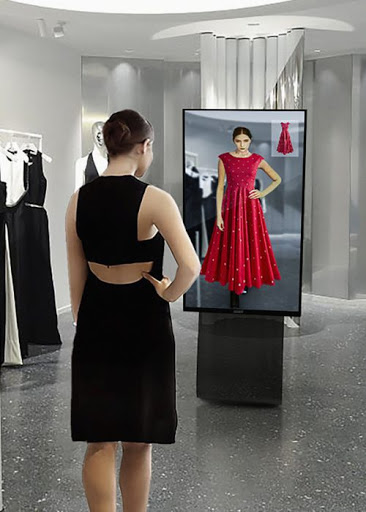
\includegraphics[width=0.3\textwidth]{fit-ar.jpg}
    \caption{Virtual Dressing Room \cite{vdr}}
\end{figure}

Nowadays, people are purchasing most of their items online and are spending more on it especially in fashion items since browsing different styles and categories of clothes is easy with just a few mouse clicks. Despite the convenience that online shopping provides, customers tend to concern about how a particular fashion item image on the website would fit with themselves. Therefore, there is an urgent demand to provide a quick and simple solution for virtual try-on. Instead of using 3D information such as depth of the image, we believe simply rely on the regular 2D photo is the most convenient way to satisfy this need. With the recent progress in virtual try-on technologies, people can have a better online shopping experience by accurately envisioning themselves wearing the clothes from online categories. Furthermore, virtual try-on technologies not only have demand in online shopping but also in physical shopping. In other words, with the try-on technologies developed on mobile application, customers can save their time of going into the fitting room.

\section{Background}\label{background}

Seminal work on virtual fitting with traditional computer vision techniques is DRAPE \cite{guan2012drape}. DRAPE model is trained with meshes of pose of person and shapes of clothes. They utilized \textit{shape deformation gradients}, a linear transformation function that aims to align triangles from source and target mesh, to represent deformation between meshes. DRAPE applied the process of deformation due to body shape, rigid part rotation, and body pose. Recent advances in machine learning, in particular, deep neural networks forwards the performance of virtual try-on systems significantly. VITON \cite{han2018viton} is a virtual try-on network with an encoder-decoder generator as its core component. Instead of accessing 3D information such as in previous techniques \cite{guan2012drape}, VITON only leveraged 2D information in its virtual try-on network. Therefore, VITON reduces the resource footprint and enables a broader set of applications. State-of-art methods such as ClothFlow \cite{han2019clothflow} outperforms VITON by extending the networks in VITON. In particular, ClothFlow divides the try-on framework into three stages. (1) target segmentation map generation. (2) refinement of geometric information in a cascaded warping manner. (3) synthesis of the final result. These extra stages are shown to improve the synthesis of photo-realistic images. In our study, we do not plan to evaluate DARPE against recent deep learning approach such as VITON since DARPE requires 3D meshes whereas VITON is targeted toward 2D image. Instead, although not direcrtly related to your topic, we found a project named E-dressing in the public domain which relies on traditional machine learning techniques to realize virtual fitting room.  

\section{Evaluation}\label{eval}

We will run VITON and test its performance on our own dataset crawled by the web crawler we developed and examine the VITON's reproducibility. On the other hand, we will investigate non-neural network techniques for performing the task of virtual fitting.

We will apply the evaluation methods described by Han et al in \cite{han2018viton}. In particular, we will use the VITON dataset we found online and we will measure the inception score for both traditional techniques and deep learning approach proposed in VITON.
Inception score is usually used to quantitatively evaluate the synthesis quality of image generation models. Higher inception scores indicate the evaluated model can produce visually diverse and semantically meaningful images which demonstrates the generality of a given machine learning approach. 

\section{Deliverables \& Milestones} \label{dev-stone}

Our plan is to start by investigating traditional computer vision methods such as image stitching we learned in class and papers such as DRAPE \cite{guan2012drape} and gradually move onto newer approaches such as deep learning-based techniques. We will try to use pre-trained model if provided for each methods before we try to re-implement the best or current state-of-the-art method.

% dax go go go
% dax zZZ zZZ
% 739 做實驗
\begin{itemize}
    \item 2/21: Read and research some more papers. Create a webpage or a shared media for documenting the project.
    \item 3/13: Finish investigations for traditional CV (DRAPE) vs. VITON / VITON-GAN vs. ClothFlow.
    \item 3/20: Start some re-implementation of state-of-the-art paper.
    \item 3/31: Finish Project Mid-Term Report.
    \item 4/10: Finish re-implementation and start evaluation and comparison for different datasets (VITON vs DeepFashion). Find ways to improve existing solutions.
    \item 4/27, 4/29, or 5/1: Wrap-up and finish slides for Final Project Presentations
    \item 5/4: Finish Project Webpage.
\end{itemize}

\section{Midterm Report} \label{mid-report}

\subsection{E-Dressing} 
We investigated E-Dressing \footnote{\url{https://github.com/iamsusmitha/E-Dressing}} which is a system that uses traditional machine learning methods, in particular, an ensemble of regression trees \cite{kazemi2014one}, to perform the tasks of virtual try-on. However, after experimenting with the system and running author-provided demos, we would argue that E-Dressing is limited to try-on of items on faces. For example, glasses and earrings. Although this does not align with our original plan of the project, we see the possibility of integrating this feature into our final system to have a full-body try-on feature since CP-VTON (as described below) only support try-on of shirts. We will continue our investigation of using traditional machine learning methods for virtual try-on as the project progresses. Since the outcome of E-Dressing is a bit disappointing, we spend the majority of our time on CP-VTON as described below.

\subsection{Data Preparation and Pre-Processing}
In order to gather data for training and evaluation purposes. We have implemented a scraper to scrape clothes images from E-Commerce websites. After scraping the images, we found 2 major problems.

First, the clothes images are mixed with clothes only, clothes on model front/side/back, detailed parts of the clothes, or even different clothing combinations on the model, etc. We haven't find out an automated way to pick out only the high quality clothes-only images yet, but we plan to try out existing image classification services.

Second, most clothes images comes with background, and for our model we need the background-removed image with a binary mask. Therefore, we investigated and tried implementing several background-removal techniques.

\subsubsection{Scraper for Clothes Images}
We used Scrapy with Python and implemented a website crawler and scraper. In particular, we targeted the E-Commerce website https://uniqlo.com and scraped for their women's T-shirt images.

The major problem we faced here (aside from the two mentioned above) is that the amount of women's T-shirts from any single seller is very little, often only around a few hundred. If we want to get a large amount of high-quality data, this method would not scale well.

\subsubsection{Image Background Removal}
In order to remove background from images, we investigated both traditional-CV methods and Machine-Learning methods. We found out that although Machine-Learning methods generally performs better results, it only works well on the same subject when it was trained. For example, a library we tested\footnote{\url{https://github.com/aadityavikram/Background-Removal}} which uses 100 layers of Tiramisu DensNet trained on images with person works well on removing background from images that contain one person, but performs terribly on even really easy t-shirt-only images (Figure \ref{fig:bgrm-ml}).

\begin{figure}[H]
    \centering
    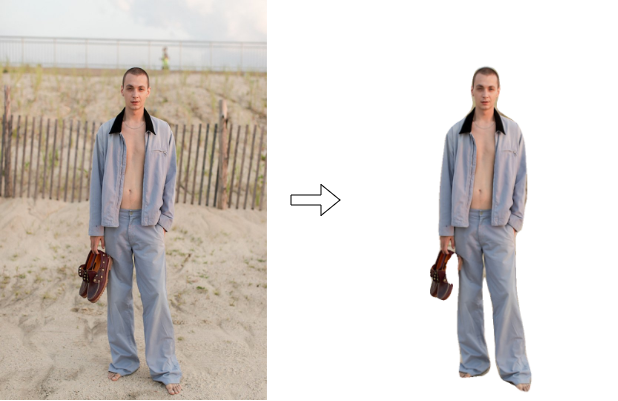
\includegraphics[width=1\textwidth]{rmbg/ml-person.png}
    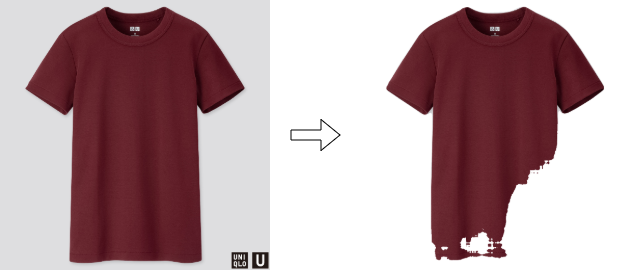
\includegraphics[width=1\textwidth]{rmbg/ml-tshirt.png}
    \caption{Background Removal using Machine Learning methods}
    \label{fig:bgrm-ml}
\end{figure}

Next we tried using traditional-CV methods for image background removal. Specifically, we tried using Canny edge detection algorithm and Otsu's thresholding algorithm, using OpenCV. The main problem is that although this works reasonably well on some easy cases (clean monotonic background with contrasted-colored t-shirt), it is hard to tune the thresholds for every kind of t-shirt to have clean results.

We have created a simple web page\cite{opencvjswebsite} (online demo\footnote{\url{https://opencv-js-background-removal.netlify.com/}}) using OpenCV.js, in order to visualize the effect of tuning Brightness/Contrast together with comparing two algorithms mentioned above, and to visually check each steps output to further improve the algorithm pipelines. On this web page, we can test out different clothes and change their brightness/contrast and toggle pipeline such as morphing steps to see how they affect the generated contours and masks. The screenshot result for the same easy t-shirt-only is shown in Figure \ref{fig:bgrm-cv}.

\begin{figure}[H]
    \centering
    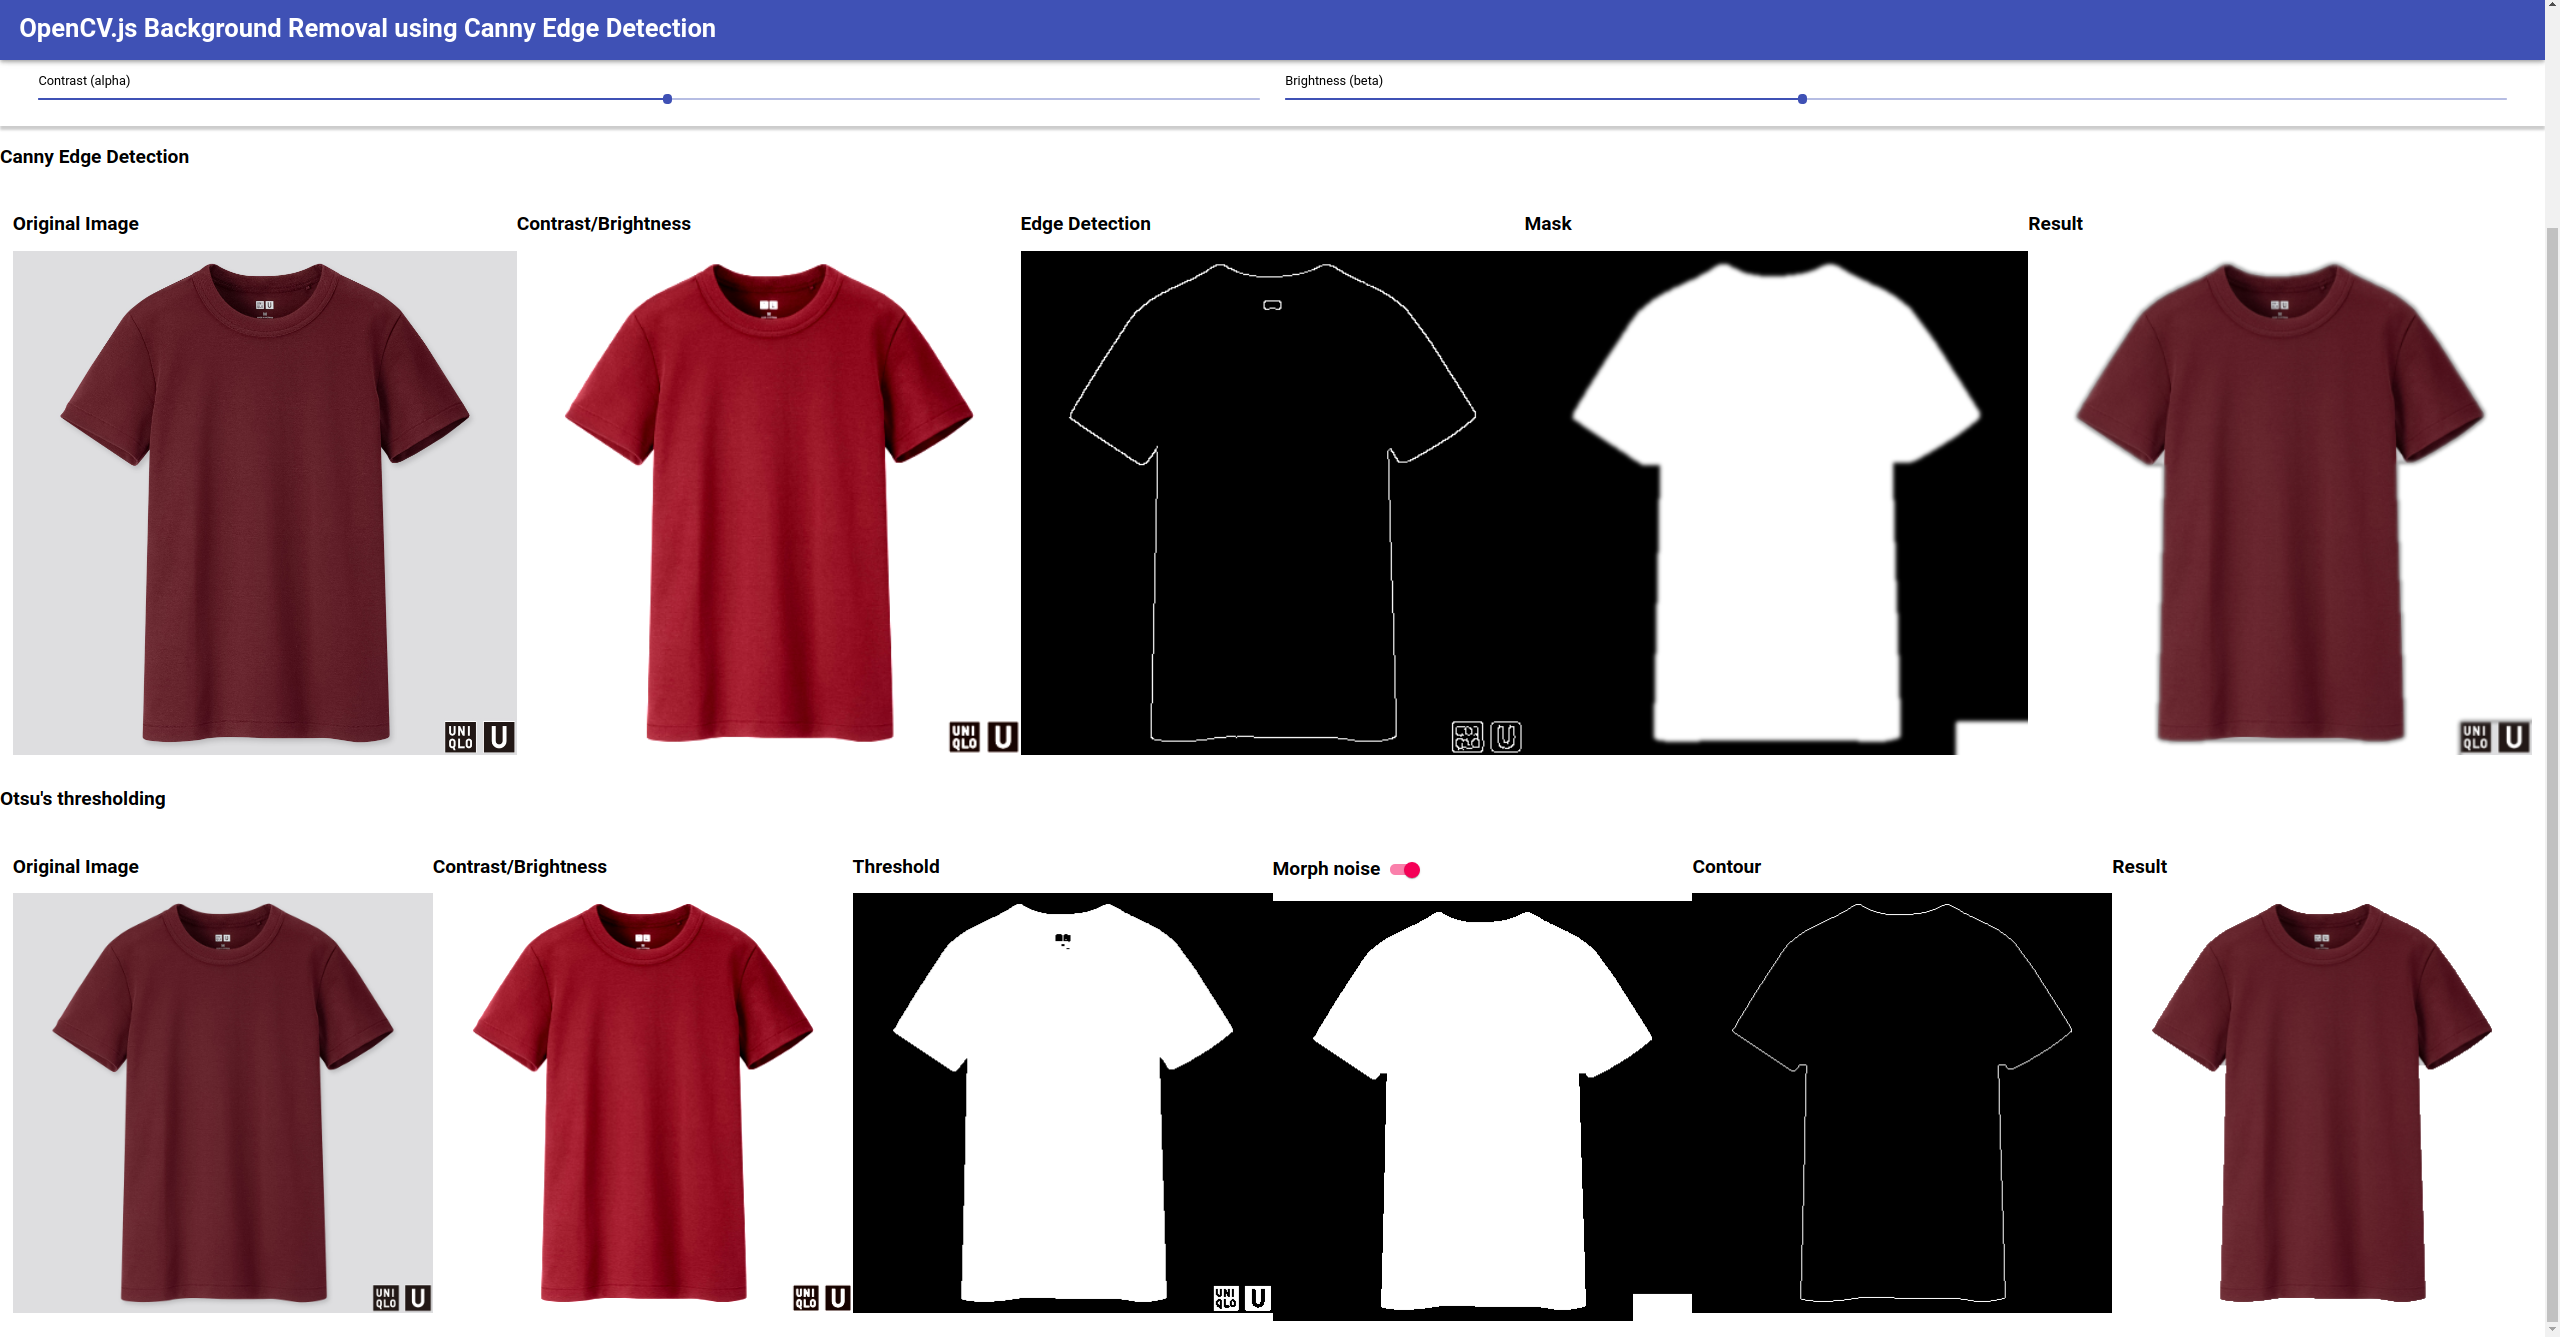
\includegraphics[width=1\textwidth]{rmbg/cv-tshirt.png}
    \caption{Screenshot for website\cite{opencvjswebsite} to test background removal using traditional CV methods}
    \label{fig:bgrm-cv}
\end{figure}

Images with more complex colors, lower contrast between clothes and backgrounds, more shadows, etc. is still problematic and needs to be improved.

\subsection{CP-VTON}
We've reimplemented the paper (Toward Characteristic-Preserving Image-based Virtual Try-On Network) method using the same dataset and model settings.

\subsubsection{Dataset \& Preprocessing}
For the dataset, we use the same data provided by original VITON \& CP-VTON \footnote{\url{https://drive.google.com/open?id=1MxCUvKxejnwWnoZ-KoCyMCXo3TLhRuTo}}, which use OpenPose\cite{cao2018openpose} for JSON format pose information, and LIP\_JPPNet\cite{liang2018look} for model image segmentation.

\subsubsection{Methodology}
In CP-VTON, they use a two-stage solution to deal with the virtual try-on problem. First, it learns a transformation for transforming the clothes into fitting the body shape of the target person via a new Geometric Matching Module (GMM). Second, to mitigate edge artifacts of warped clothes and make the results more realistic, CP-VTON applies a Try-On Module (TOM) that learns a combination mask to integrate the warped clothes and the  rendered image to ensure smoothness.\\

\textbf{Geometric Matching Module (GMM)}
    \begin{itemize}
        \item input: Person Representation $p$ (Keypoints + Segmentation + Human Model Image) + Cloth $c$
        \item output: Warped Clothes $c'$
        \item loss function: $L_{1}$ loss
    \end{itemize}
\textbf{Try-On Module (TOM)}
    \begin{itemize}
        \item input: Person Representation $p$ (Keypoints + Segmentation + Human Model Image) + Warped Clothes $c'$ (generated by GMM)
        \item output: Human Model with warped cloth
        \item loss function: $L_{1}$  + $L_{VGG}$ loss
    \end{itemize}
\begin{figure}[H]
    \centering
    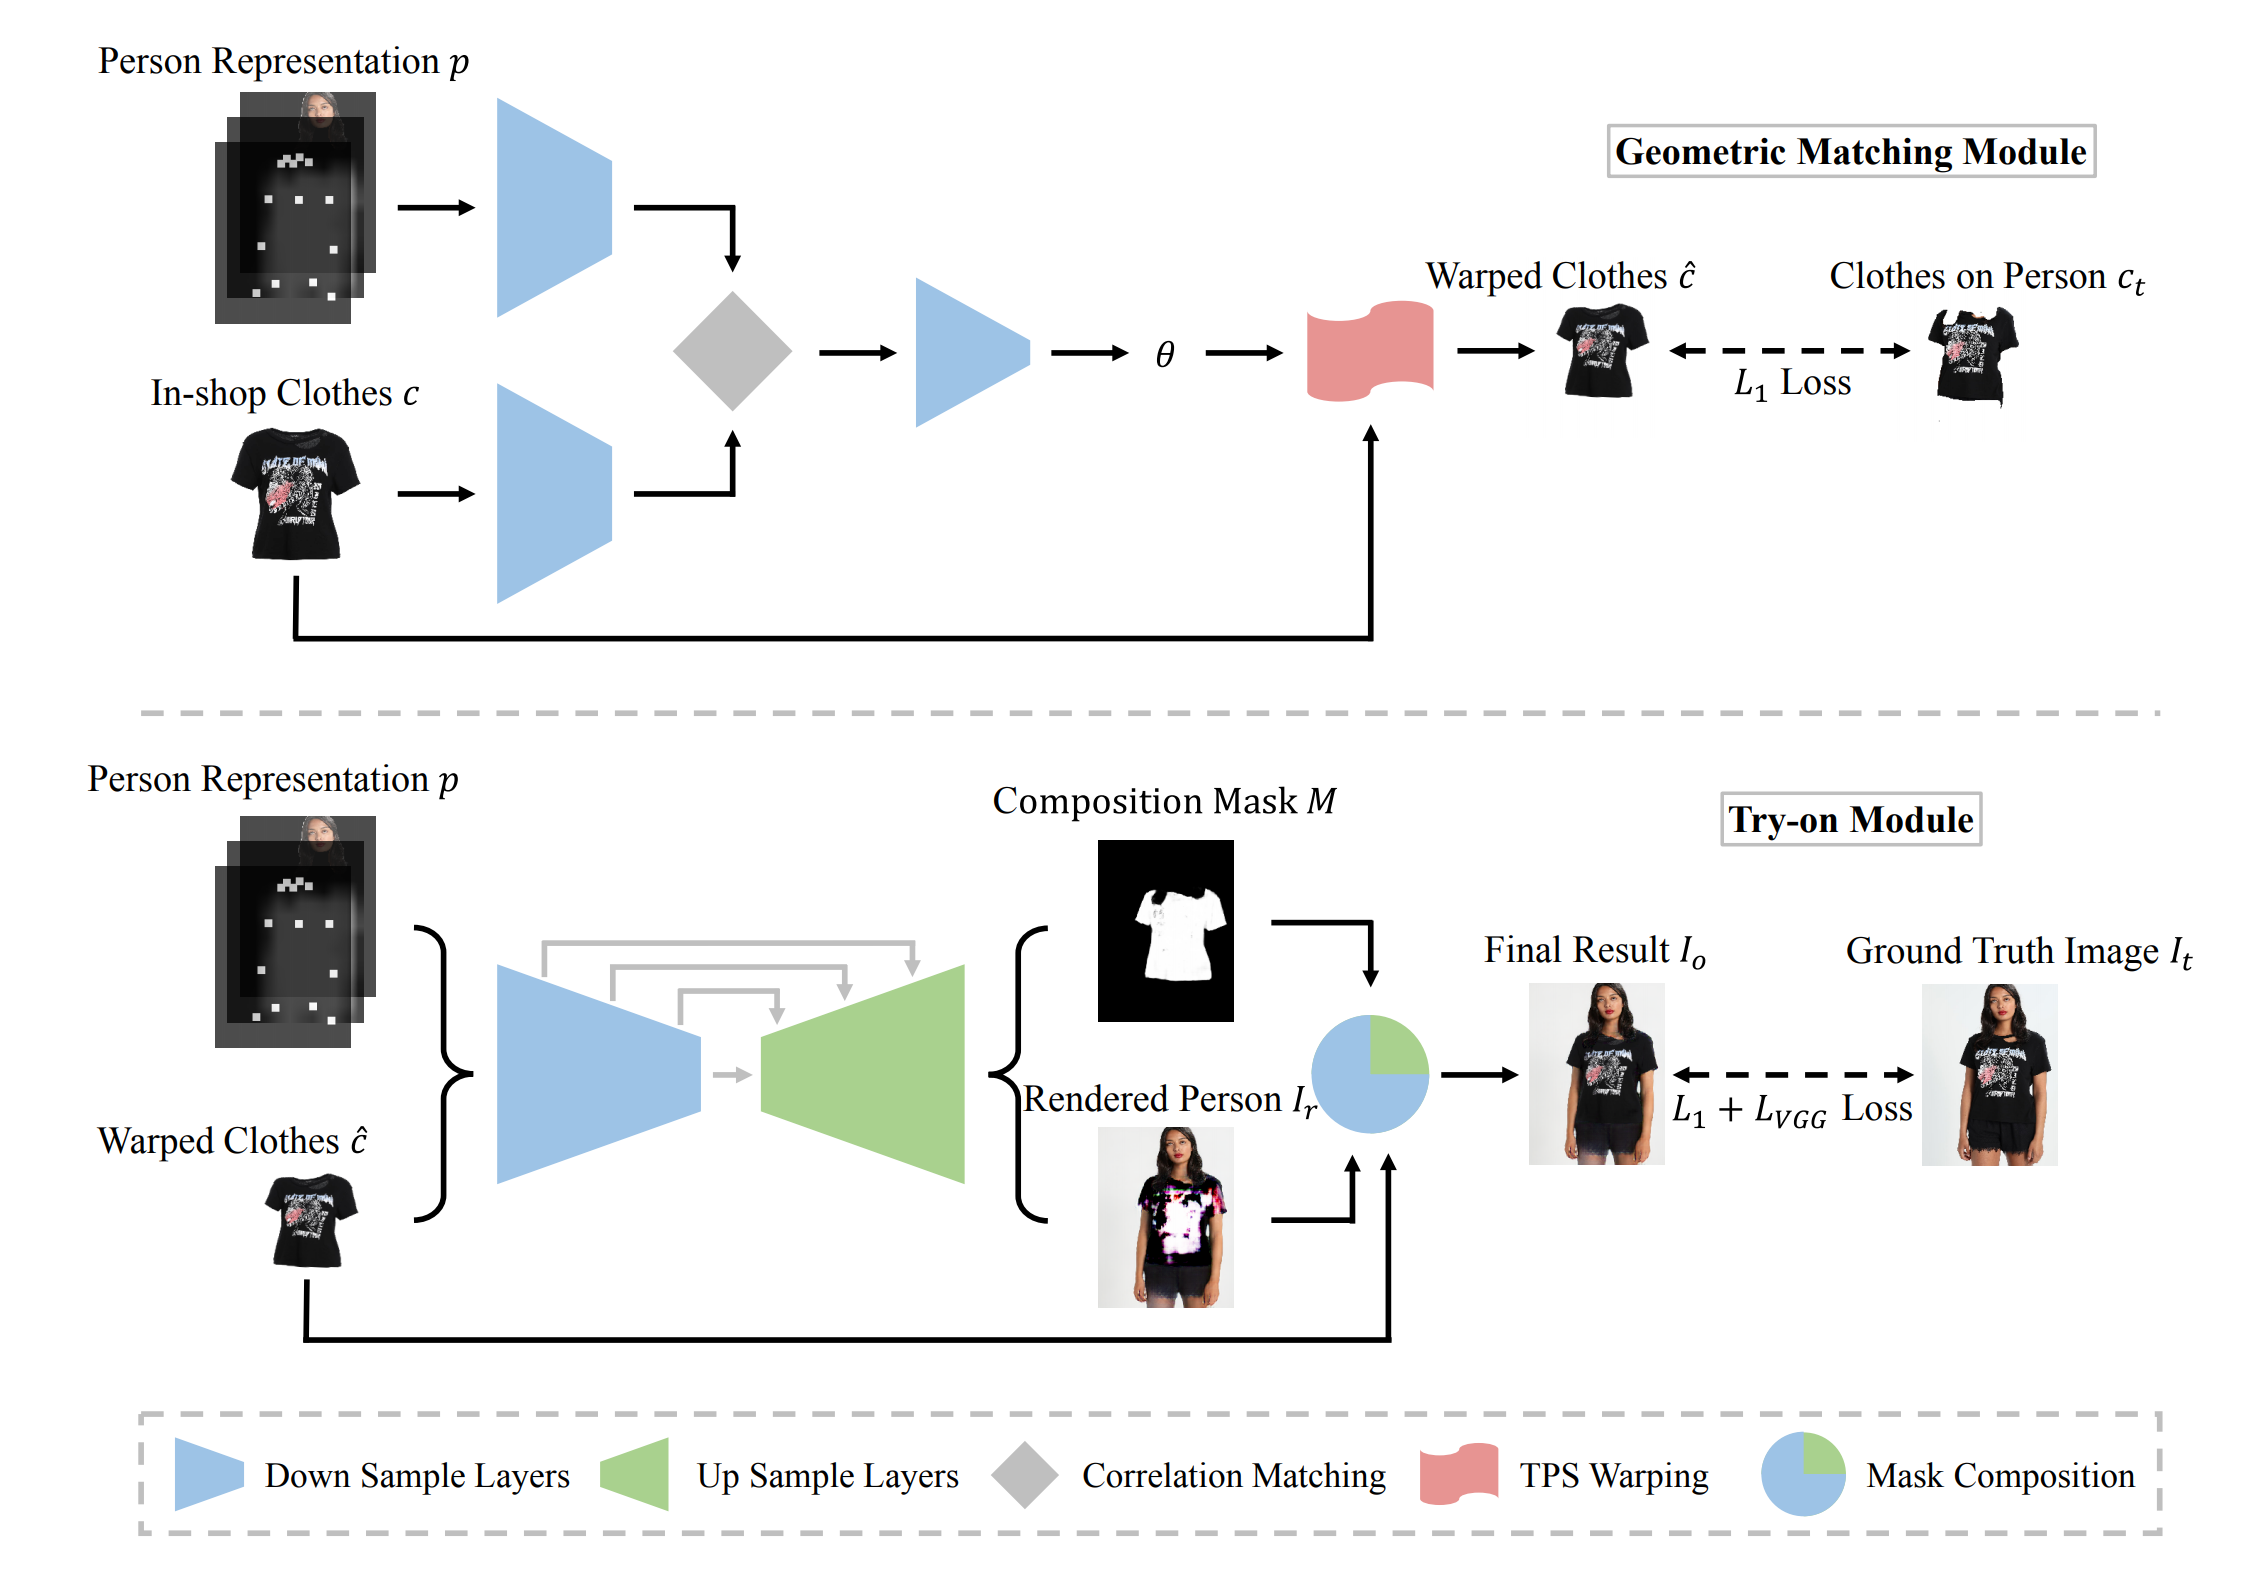
\includegraphics[width=1\textwidth]{cp-vton-imgs/CP-VTON-Model.png}
    \caption{Overview of CP-VTON}
    \label{fig:cp-vton}
\end{figure}

\subsubsection{Evaluation} 
We use provided dataset to evaluate the model result in Figure \ref{fig:provided}. Furthermore, we use our own data (Cloth + Human Model Image) to see the model effect in Figure \ref{fig:our}.

We can see better try-on results in the provided dataset compared to using our dataset. We guess it is due to the difference between training and testing dataset properties. Since we crawl our dataset on the Internet and doing minor preprocess (crop and resize), many aspects can affect the original model inference such as image quality, background removal, cloth texture varies in brands and so on. Moreover, we notice that there's a limitation using CP-VTON i.e. it will transfer Human Model's pants into different texture or even color.

\begin{figure}[H]
    \centering
    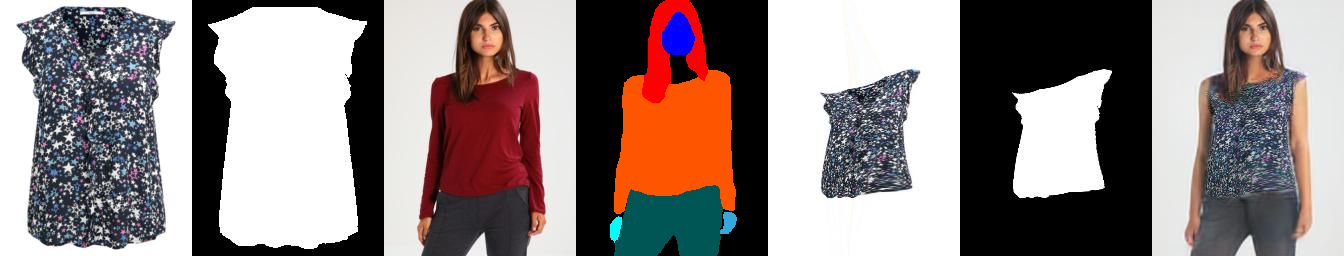
\includegraphics[width=1\textwidth]{cp-vton-imgs/visual1.png}
    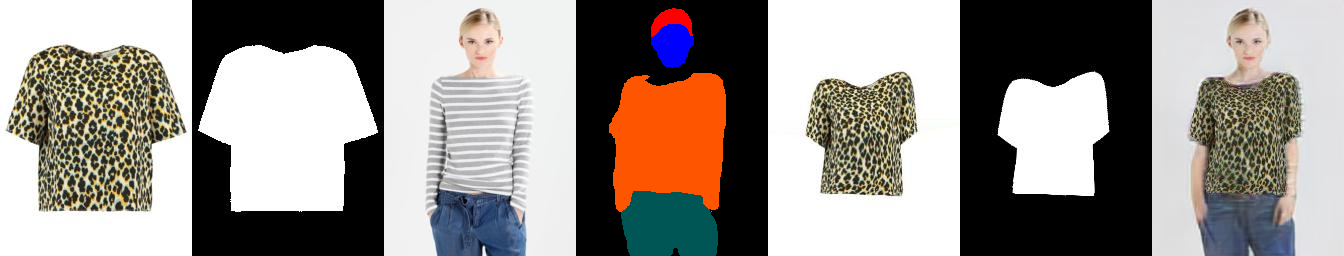
\includegraphics[width=1\textwidth]{cp-vton-imgs/visual2.png}
    \caption{Evaluation of cp-vton using provided dataset}
    \label{fig:provided}
\end{figure}

\begin{figure}[H]
    \centering
    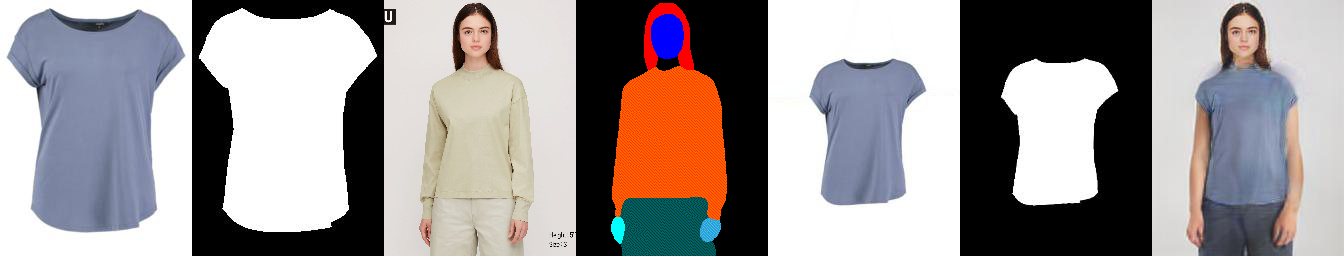
\includegraphics[width=1\textwidth]{cp-vton-imgs/src_a_dst_018746.png}
    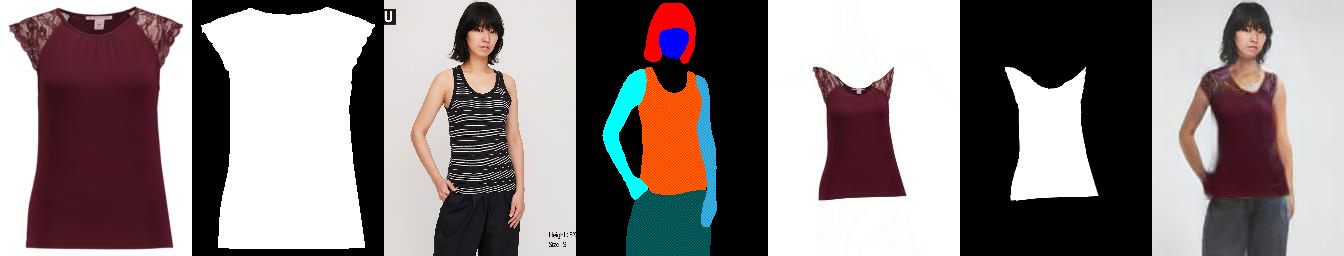
\includegraphics[width=1\textwidth]{cp-vton-imgs/src_b_dst_005053.png}
    \caption{Evaluation of cp-vton using our dataset}
    \label{fig:our}
\end{figure}



\printbibliography
\end{document}
